

\chapter{نمودار کلاس تحلیل}
\label{chapter:classAnalysis}

در ادامه نمودار کلاس‌های تحلیل قرار گرفته است. در شکل اولیه نمودار‌ها ارتباط‌های Association بین کلاس‌ها به دلیل شلوغ نشدن قرار نگرفته است و در شکل آخر این ارتباط‌ها آورده شده‌اند.


\begin{figure}[ht!]
	\centering
	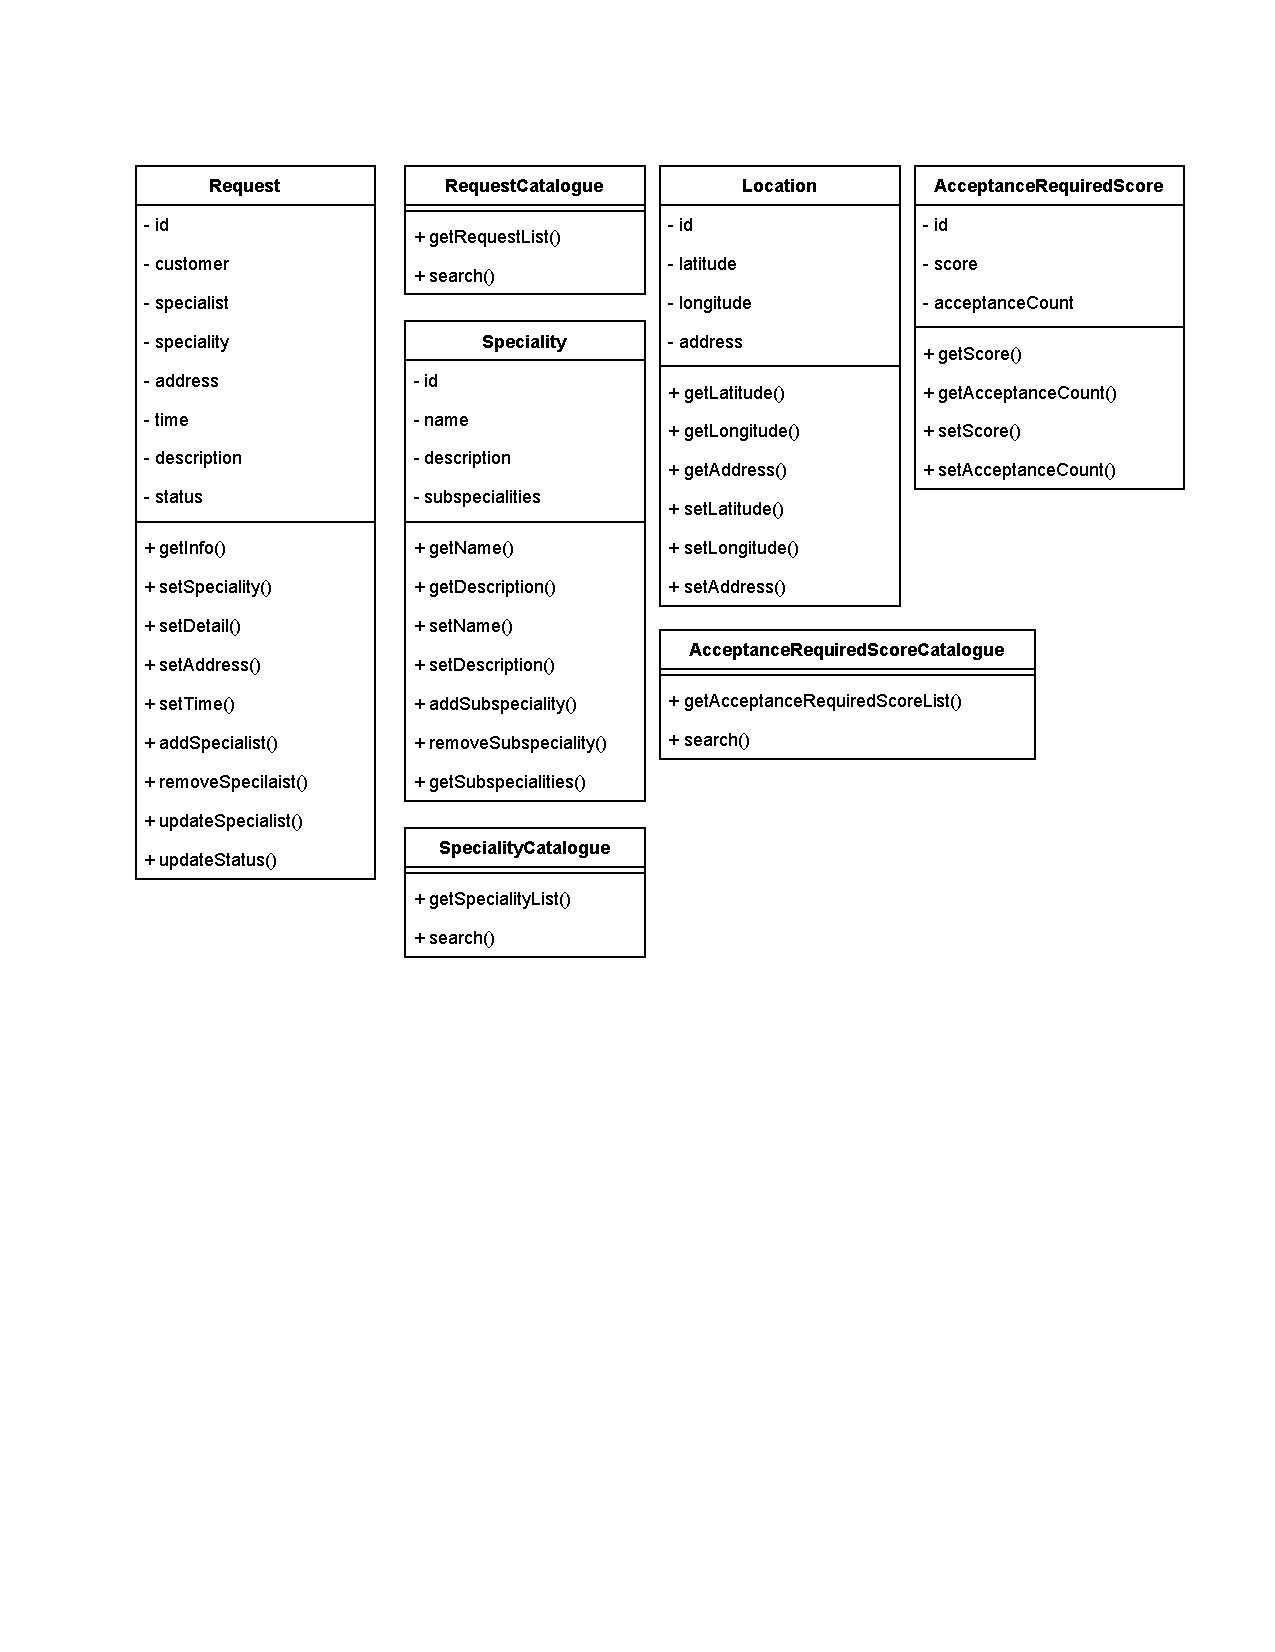
\includegraphics[scale=0.8]{figs/OOD-class-page-1.pdf}
	\caption{نمودار کلاس: کلاس‌های طراحی بخش اول}
\end{figure}
\FloatBarrier
\newpage


\begin{figure}[ht!]
	\centering
	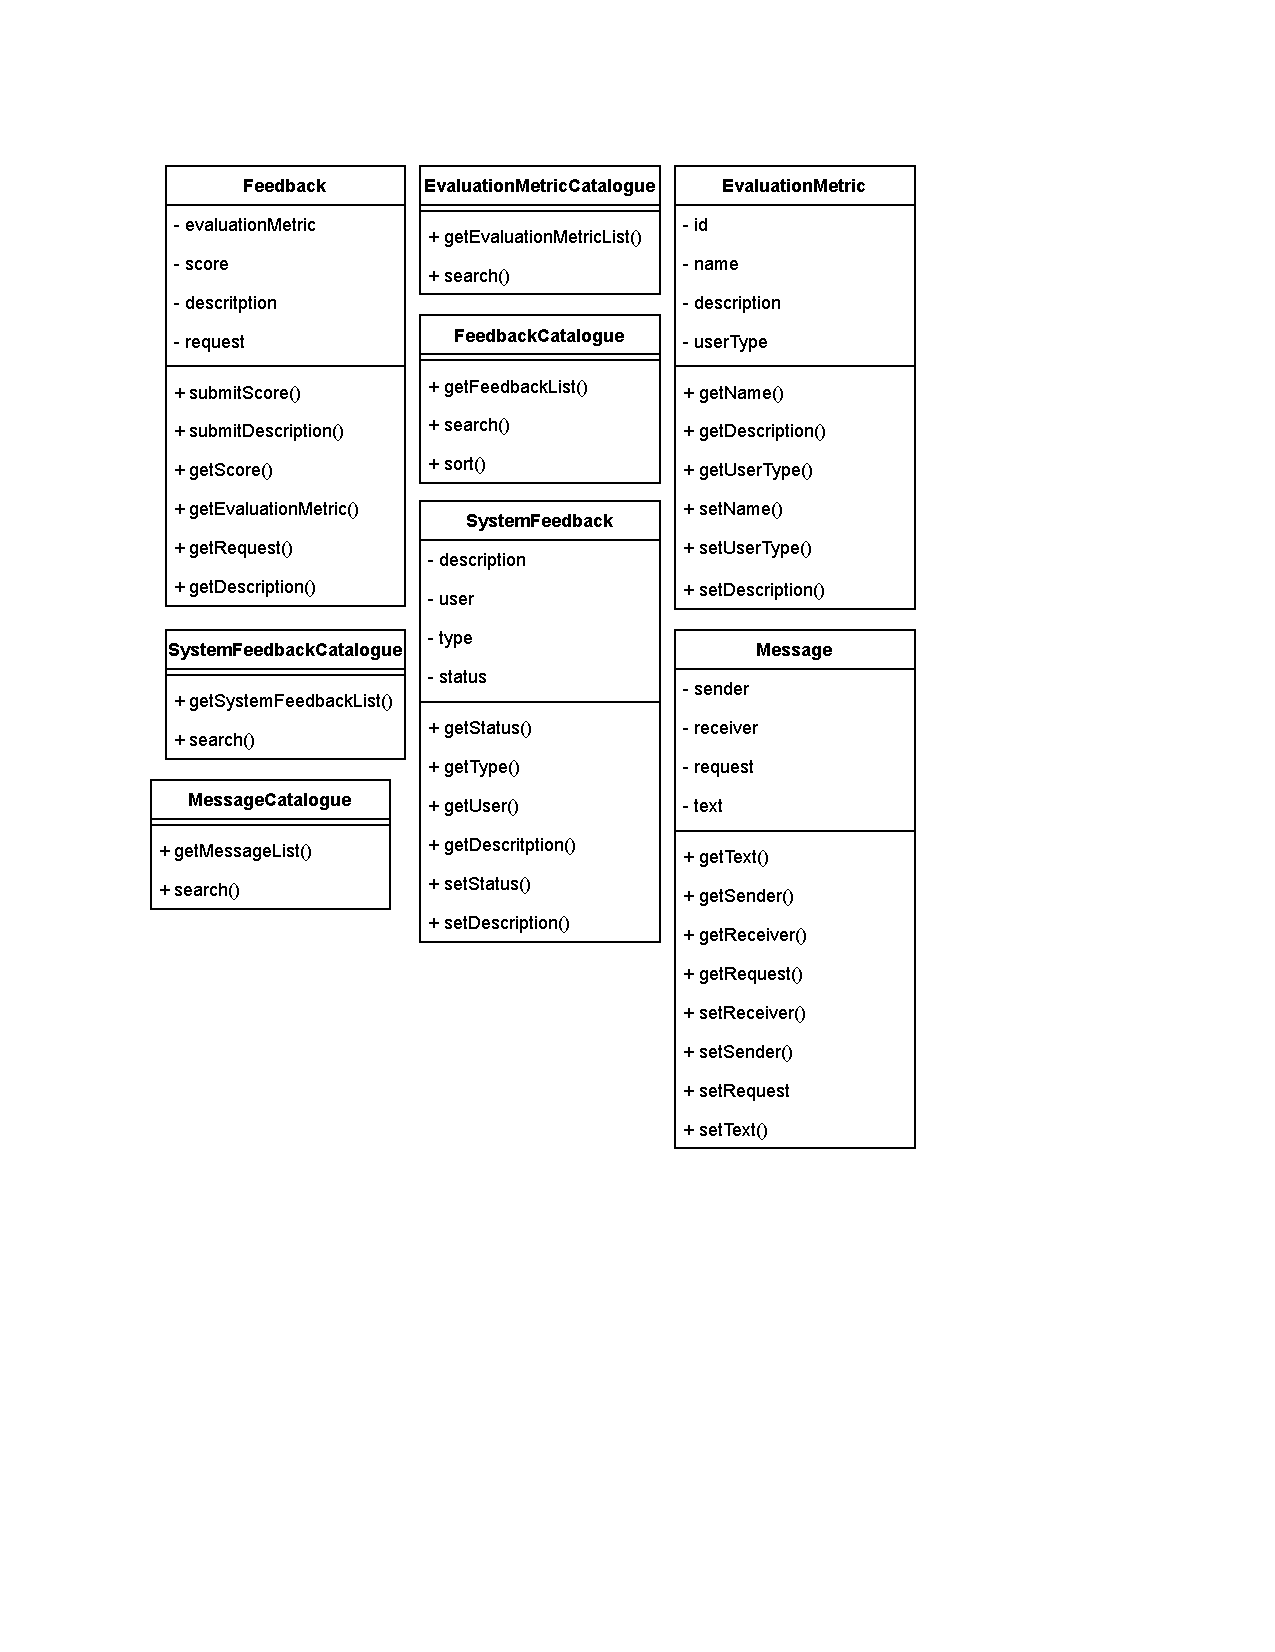
\includegraphics[scale=0.8]{figs/OOD-class-page-2.pdf}
	\caption{نمودار کلاس: کلاس‌های طراحی بخش دوم}
\end{figure}
\FloatBarrier
\newpage

\begin{figure}[ht!]
	\centering
	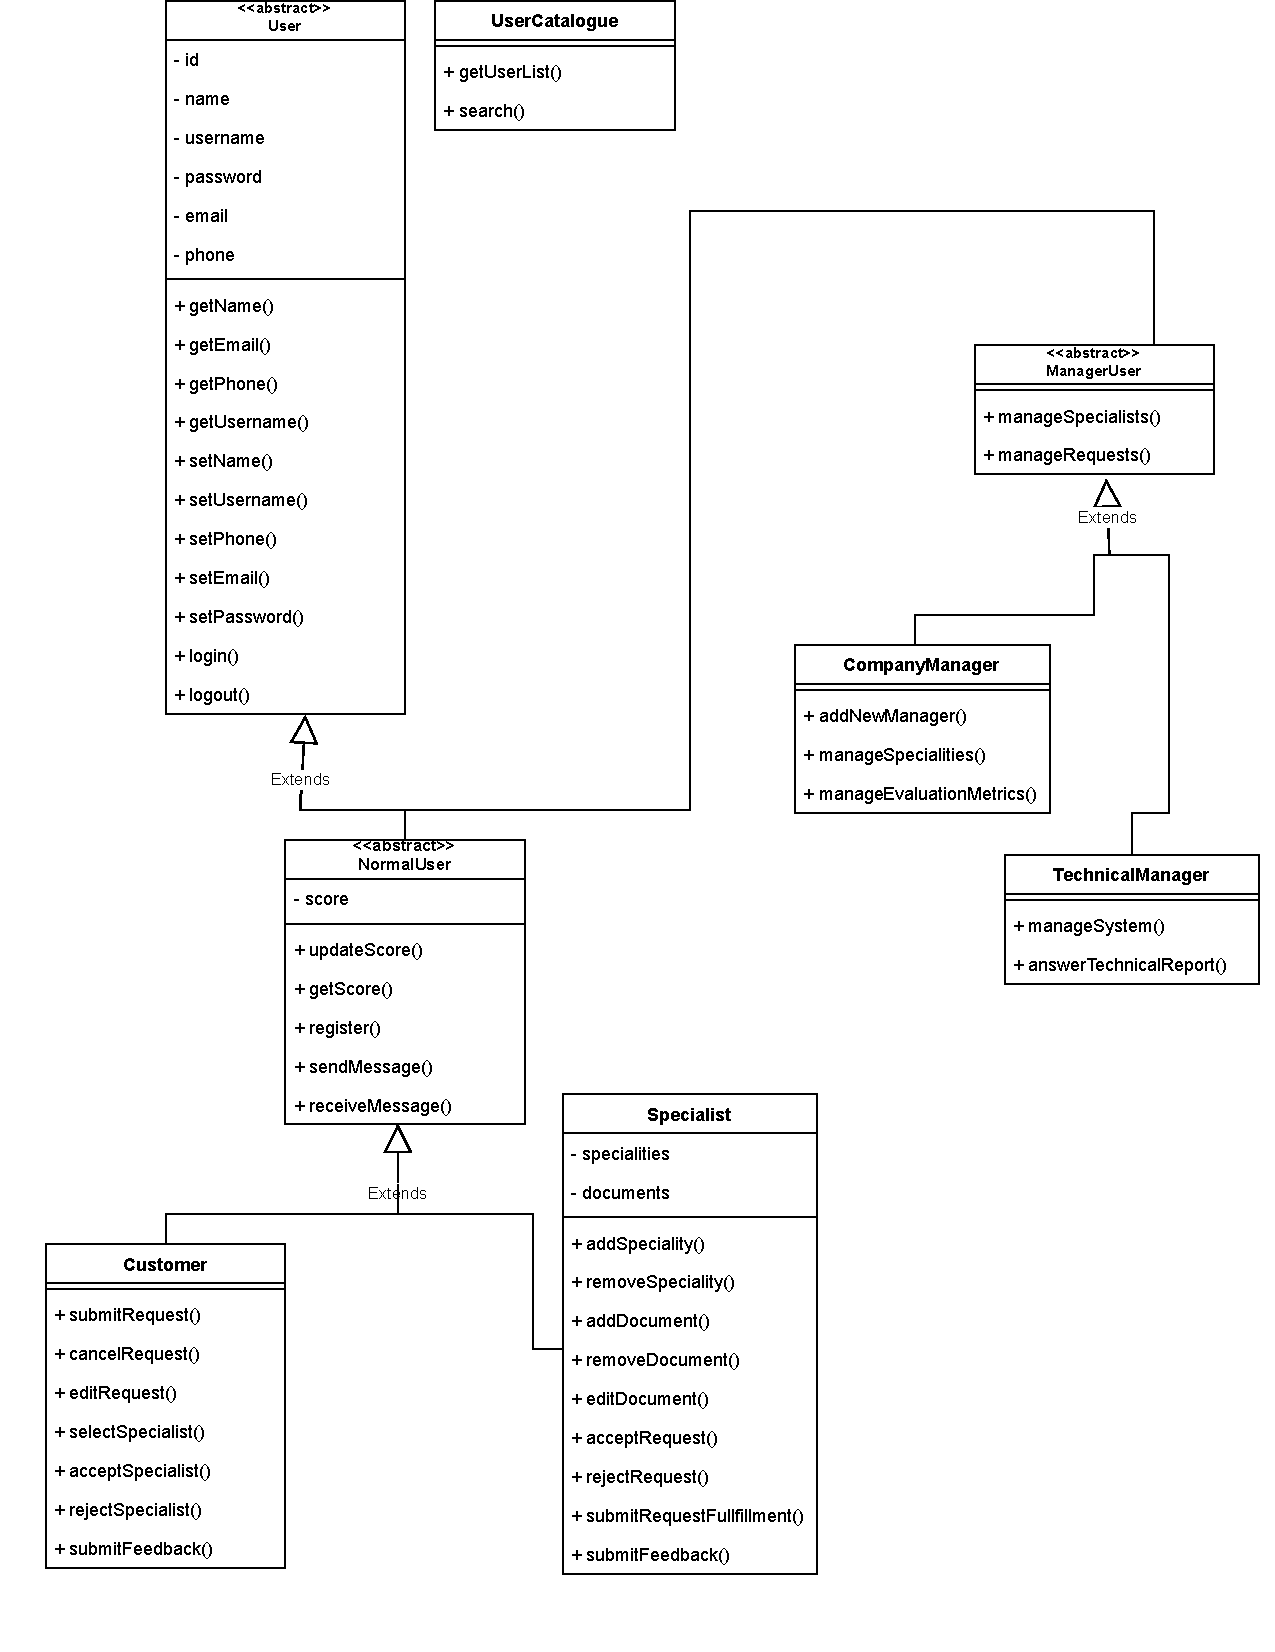
\includegraphics[scale=0.8]{figs/OOD-class-page-3.pdf}
	\caption{نمودار کلاس: کلاس‌های طراحی بخش سوم}
\end{figure}
\FloatBarrier
\newpage

\begin{figure}[ht!]
	\centering
	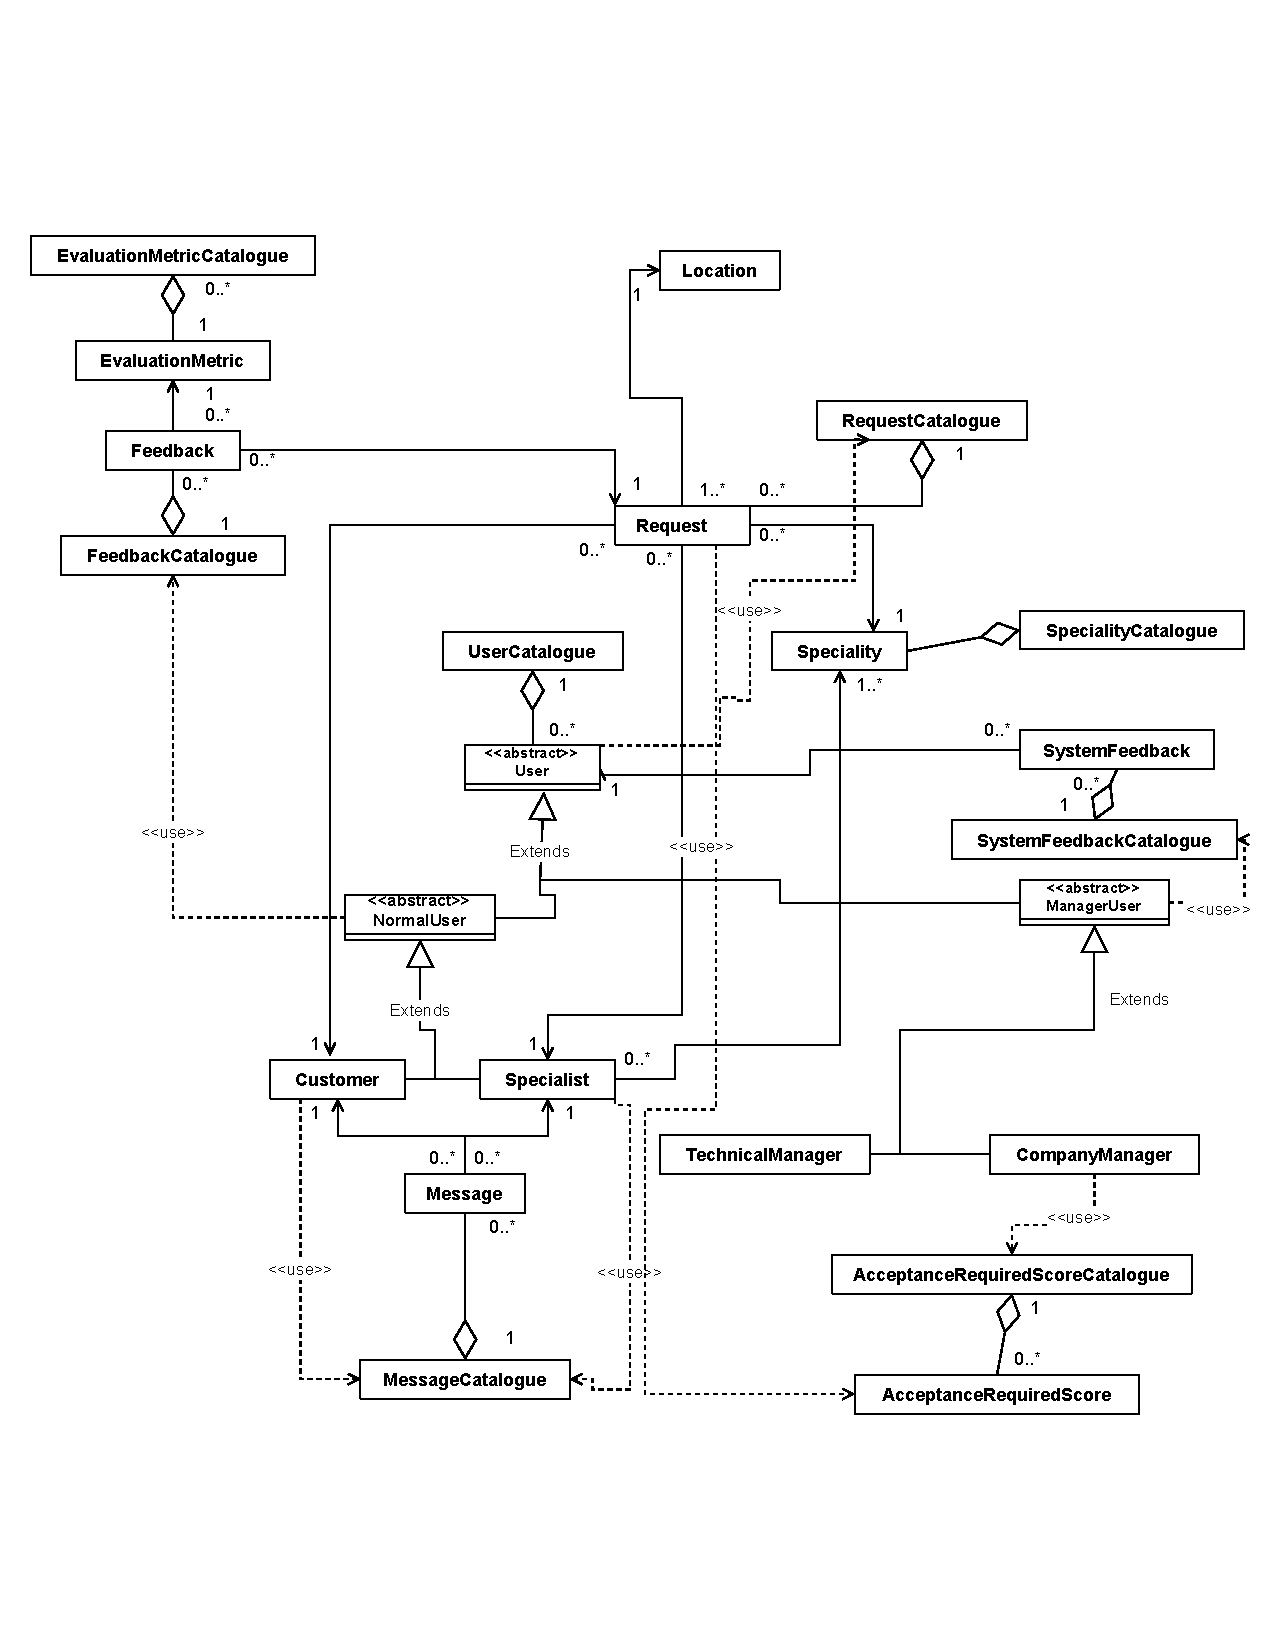
\includegraphics[scale=0.8]{figs/OOD-class-page-4.pdf}
	\caption{نمودار کلاس: ارتباط بین همه کلاس‌ها}
\end{figure}
\FloatBarrier
\newpage